\documentclass{article}
\usepackage{graphicx} % Required for inserting images
\usepackage{float} % For figures placement
\usepackage{fancyvrb} % for \Verb
\usepackage[a4paper, margin=2.5cm]{geometry}
\usepackage{karnaugh-map} % Tableau de Karnaugh
% Subfigures
\usepackage{caption}
\usepackage{subcaption}
\usepackage{multicol}

\usepackage{amsmath}
\usepackage{emoji}

\usepackage{enumitem}

\usepackage[hidelinks]{hyperref}


\usepackage{listings}
\usepackage{xcolor}

\definecolor{codegreen}{rgb}{0,0.6,0}
\definecolor{codegray}{rgb}{0.5,0.5,0.5}
\definecolor{codepurple}{rgb}{0.58,0,0.82}
\definecolor{backcolour}{rgb}{0.95,0.95,0.92}

\lstdefinestyle{mystyle}{
    backgroundcolor=\color{backcolour},   
    commentstyle=\color{codegreen},
    keywordstyle=\color{magenta},
    numberstyle=\tiny\color{codegray},
    stringstyle=\color{codepurple},
    basicstyle=\ttfamily\footnotesize\linespread{0.1},
    breakatwhitespace=false,         
    breaklines=true,                 
    captionpos=b,                    
    keepspaces=true,                 
    numbers=left,                    
    numbersep=5pt,                  
    showspaces=false,                
    showstringspaces=false,
    showtabs=false,                  
    tabsize=2,
}

\newcommand{\lstbg}[3][0pt]{{\fboxsep#1\colorbox{#2}{\strut #3}}}
% \lstdefinelanguage{diff}{
%   basicstyle=mystyle,
%   morecomment=[f][\lstbg{red!20}]-,
%   morecomment=[f][\lstbg{green!20}]+,
%   morecomment=[f][\textit]{@@},
%   %morecomment=[f][\textit]{---},
%   %morecomment=[f][\textit]{+++},
% }

\lstset{
    language=C++,
    style=mystyle,
}

\usepackage{setspace} % to change line spacing
\renewcommand{\baselinestretch}{1.5} 


\setlength{\parskip}{\baselineskip}%
\setlength{\parindent}{0pt}%

\begin{document}

\makeatletter
\begin{titlepage}
\begin{center}
    

\includegraphics[width=7cm]{assets/LogoCN_Q.png}
\\
\textbf{\large{Centrale Nantes}}
\\[2cm]

\textbf{\large{MAC : $4^{th}$ Lab's Report \\
Timers --- Stepper Motor control }}
\\[14pt]
$1^{st}$ year Embedded Systems Engineering
\\[2cm]


\vfill

\textbf{By} \\
EL KHAYDER Zakaria \\
SAOUTI Rayan
\\[1cm]

\textbf{Professor} \\
BRIDAY Mikael
\\[3cm]


December 07, 2023 \\ [12pt]

Session \\
2023-2024 \\[12pt]
\small{Made with \LaTeX}
\end{center}
\end{titlepage}
\makeatother

\pagebreak

\setcounter{page}{1}
\pagenumbering{Roman}

\clearpage
\addcontentsline{toc}{section}{Contents}
\tableofcontents

\clearpage
\addcontentsline{toc}{section}{List of Tables}
\listoftables
\addcontentsline{toc}{section}{Listings}
\lstlistoflistings

\clearpage

\setcounter{page}{1}
\pagenumbering{arabic}

\section{Counter-Clockwise Rotation}

\subsection{Setup}

\begin{lstlisting}[language=C++, caption={Motor output setup}]
void setup()
{
    // Setup Motor Output pins
    for (int i = 5; i <= 8; i++)
        pinMode(GPIOA, i, OUTPUT);
}
\end{lstlisting}

\subsection{Single step Counter-Clockwise}
\begin{lstlisting}[language=C++, caption={stepCCW()}]
#define SEQ_LEN sizeof(seq) / sizeof(*seq)

void stepCCW()
{
    static uint8_t index = 0; // Static variable to preserve its state 
    const unsigned char seq[] = {8, 0xC, 4, 6, 2, 3, 1, 9};

    GPIOA->ODR &= ~(0b1111 << 5); // Force all the 4 pins to 0
    GPIOA->ODR |= seq[index] << 5; // Set the appropriate bits to 1

    index++;
    index %= SEQ_LEN; // reset on 8
}
\end{lstlisting}

\subsection{Using a timer}

\subsubsection{Setup}

We should start by setting up the timer, for this lab, we chose to use \verb|TIM6|. \\
We chose a pre-scalar of 64000(-1), giving us an increment each 1 ms (1KHz). The chosen \verb|PSC| value makes calculating the \verb|ARR| easier with the simple equation:
$$
\verb|ARR| = \frac{1000}{f} - 1
$$

In our first run, we take $f = 10$, but the equation is available for any equation between 1 and 999.
We can inline this equation directly in code or as C++ Macro. We chose the latter.
While at it, we might define a \verb|Timer| const for \verb|TIM6|.

\begin{lstlisting}[language=C++]
#define Timer TIM6
#define ARR(f) 1000.0 / f - 1
\end{lstlisting}

For the rest of the setup function, we just copied (stole) it directly from the presentation slides.

\begin{lstlisting}[language=C++, caption={Timer setup function}]
void setup()
{
    ...

    // input clock = 64MHz.
    RCC->APB1ENR |= RCC_APB1ENR_TIM6EN;
    // reset peripheral (mandatory!)
    RCC->APB1RSTR |= RCC_APB1RSTR_TIM6RST;
    RCC->APB1RSTR &= ~RCC_APB1RSTR_TIM6RST;

    // Configure timer
    Timer->CNT = 0; // Reset CNT
    Timer->SR = 0; // Reset flags
    Timer->PSC = 64000 - 1; // Prescalar
    Timer->ARR = ARR(10);
    Timer->CR1 = 1; // Start the timer
}
\end{lstlisting}

\subsubsection{Loop}

With the timer set up, we can now continuously check if the 0th bit of the \verb|SR| flag is raised, if that is the case, we single-step the motor and reset the said flag bit.

\begin{lstlisting}[language=C++, caption={10HZ Counter-clockwise stepping loop}]
int main(void)
{
    setup();
    
    while (1)
    {
        if (Timer->SR & 1U)
        {
            Timer->SR = 0; // Reset timer overflow flag
            stepCCW();
        }
    }

    return 0;
}
\end{lstlisting}

\subsection{Ditching the ODR and welcoming the cool BSRR}

As you may have already noticed, we can't force both 1's and 0's using masking operations on the \verb|ODR| register in a single operation. That's why, a group of people, way more smarter than us, created the \verb|BSRR| register to bypass this limitation.
With some tweaks on the \verb|stepCCW| function, we can use the same already-defined \verb|seq| for the \verb|BSRR|.

\begin{lstlisting}[language=C++, caption={Migration from ODR to BSRR}]
void stepCCW()
{
    ...

//  GPIOA->ODR &= ~(0b1111 << 5); // Force all the 4 pins to 0
//  GPIOA->ODR |= seq[index] << 5; // Set the appropriate bits to 1  
    GPIOA->BSRR = seq[index] << 5 | ~seq[index] << (16 + 5);
        
    ...
}
\end{lstlisting}

\section{Clockwise rotation}

\subsection{Single step Clockwise}

This is easy, we just copy the same already defined function (\verb|stepCCW|) and just decrement the index instead of incrementing it.

\begin{lstlisting}[language=C++, caption={stepCW()}]
void stepCW()
{
    static uint8_t index = 0;
    const unsigned char seq[] = {8, 0xC, 4, 6, 2, 3, 1, 9};

    GPIOA->BSRR = seq[index] << 5 | ~seq[index] << (16 + 5);

    if (index == 0)
        index = SEQ_LEN - 1;
    else
        index--;
}
\end{lstlisting}

\subsection{Flippity-Floppity-Floop}
We can reuse the same code from the previous lab to get the Button state, and we can reverse the rotation direction accordingly.

\subsubsection{Issue}
Now that we have two separate functions, we need a way to share the current rotation command index, to avoid distant jumps of the motor. We found that creating a global variable named \verb|RotationIndex| is the most straightforward.

\subsubsection{Reading the button state}

\begin{lstlisting}[language=C++, caption={Button setup}]
#define Button GPIOB, 1

void setup()
{
    ...

    pinMode(Button, INPUT_PULLUP);
}

\end{lstlisting}


\begin{lstlisting}[language=C++, caption={Button state}]
enum class ButtonState
{
    Released,
    Pushing,
    Pushed,
    Releasing,
};

ButtonState getButtonState()
{
    static ButtonState state = ButtonState::Released;

    switch (state)
    {
    case ButtonState::Released:
        if (digitalRead(Button) == 0) // The button is active low
            state = ButtonState::Pushing;
        break;

    case ButtonState::Pushing:
        state = ButtonState::Pushed;
        break;

    case ButtonState::Pushed:
        if (digitalRead(Button) == 1)
            state = ButtonState::Releasing;
        break;

    case ButtonState::Releasing:
        state = ButtonState::Released;
        break;
    }

    return state;
}
\end{lstlisting}

\subsubsection{Loop}

We update the main loop to check if the button is clicked, it rotates clockwise if that is the case, counter-clockwise otherwise.

\begin{lstlisting}[language=C++, caption={Rotation direction based on button state}]
int main(void)
{
    ...
    
//  stepCCW();
    if(getButtonState() == Button::Pushed)
        stepCW();
    else
        stepCCW();
    ...
}
\end{lstlisting}

\section{Rotation Speed}

\subsection{Reading the potentiometer}

Thanks to the provided \verb|adc.h/c|, the task is easy enough.

\begin{lstlisting}[language=C++]
void setup()
{
    ...
    
    ADCInit(); // Setup ADC
}
\end{lstlisting}

\begin{lstlisting}[language=C++]
int main(void)
{
    ...
    
    uint16_t value = ADCRead();
}
\end{lstlisting}

Moving along...

\subsection{Updating rotation frequency}

The potentiometer value is coded on 12 bits, meaning it goes from 0 to 4095. We can use a simple mathematical formula to map this range from 0/4095 to 10/500

$$
f = (500 - 10) \cdot \frac{v}{4096} + 10
$$

\begin{figure}[H]
    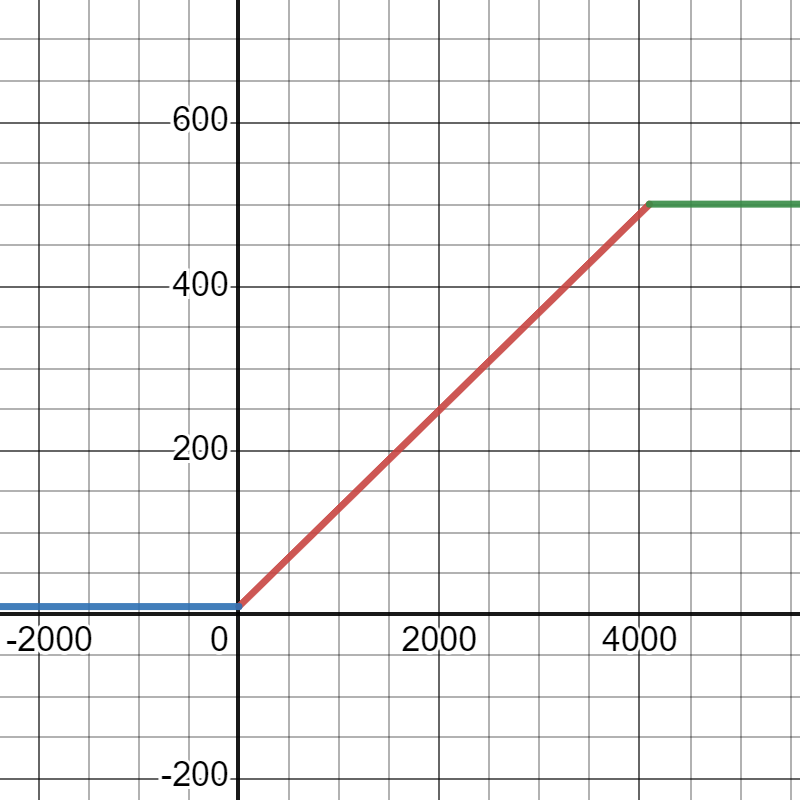
\includegraphics[width=8cm]{assets/desmos-graph.png}
    \centering
    \caption{Rotation frequency (f) $\propto$ Potentiometer value (v)}
\end{figure}

This can be easily translated to code in a single line

\begin{lstlisting}[language=C++, caption={f $\propto$ v}]
int main(void)
{
    ...

    while(1)
    {
        ...
        
        Timer->ARR = ARR(10. + (500. - 10.) * (float)ADCRead() / 4096.);
    }

    ...
}
\end{lstlisting}


\subsection{Flippity-Floppity-Floop: The sequel}
We will need a way to save the current rotation direction, and then instead of checking if the button is \verb|Pushed|, we check if it is \verb|Pushing|.

\begin{lstlisting}[language=C++]
enum class Direction
{
    Clockwise,
    CounterClockwise
};

int main(void)
{
    ...
    
    Direction direction = Direction::Clockwise;


    while(1)
    {
        if (getButtonState() == ButtonState::Pushing)
        {
            // Invert rotation direction
            if (direction == Direction::Clockwise)
                direction = Direction::CounterClockwise;
            else
                direction = Direction::Clockwise;
        }

        if (Timer->SR & 1U)
        {
            ...
            
            if (direction == Direction::Clockwise)
                stepCW();
            else // direction == Direction::CounterClockwise
                stepCCW();
                
            ...
        }
    }

    ...
}
\end{lstlisting}

\section{Tour de France}

There are 64 steps for each round, but there is also a reduction factor of 64. Meaning, that for each rotation, we should step $64 \cdot 64 = 4096$ steps.

We will need a way to keep track of the remaining steps to do. We will create a variable that we increment each time we do a step, and once it reaches the max amount (4096), we do not execute the stepping code. 

Now each time we click the button, besides only inverting the rotation direction, we should also reset the steps counter to 0

\begin{lstlisting}[language=C++, caption={What goes around... comes around}]
#define FullRoundSteps 64 * 64

int main(void)
{
    ...
    
    int rotatedSteps = 0;

    while (1)
    {
        ...

        if (getButtonState() == ButtonState::Pushing)
        {
            // Reset remaining steps
            rotatedSteps = 0;

            ...
        }
    
        if (Timer->SR & 1U)
        {
            ...
            
            if (rotatedSteps < FullRoundSteps)
            {
                ...

                rotatedSteps++;
            }
        }
    }

    return 0;
}
\end{lstlisting}

\section*{Resources}
\addcontentsline{toc}{section}{Resources}
The code files, and this report's source code, are available on this GitHub repository: \href{https://github.com/elkhayder/sec1-tp-mac}{elkhayder/sec1-tp-mac} 

\end{document}

\end{document}
 